\section{Method}

\subsection{Machine learning pipeline}
Opt 1:
\par
To solve the problem of anomaly detection and image classification, a machine learning pipeline has been developed. The pipeline consists of a anomaly detection procedure that use an autoencoder to reconstruct an input image, calculate the reconstruction error and make a decision based on the error. Images that the anomaly detection procedure considers as anomalies are then passed to a CNN to classify the anomaly. The pipeline is visualized in figure \ref{fig:ml_pipeline}.
\begin{figure}[H]
    \centering
    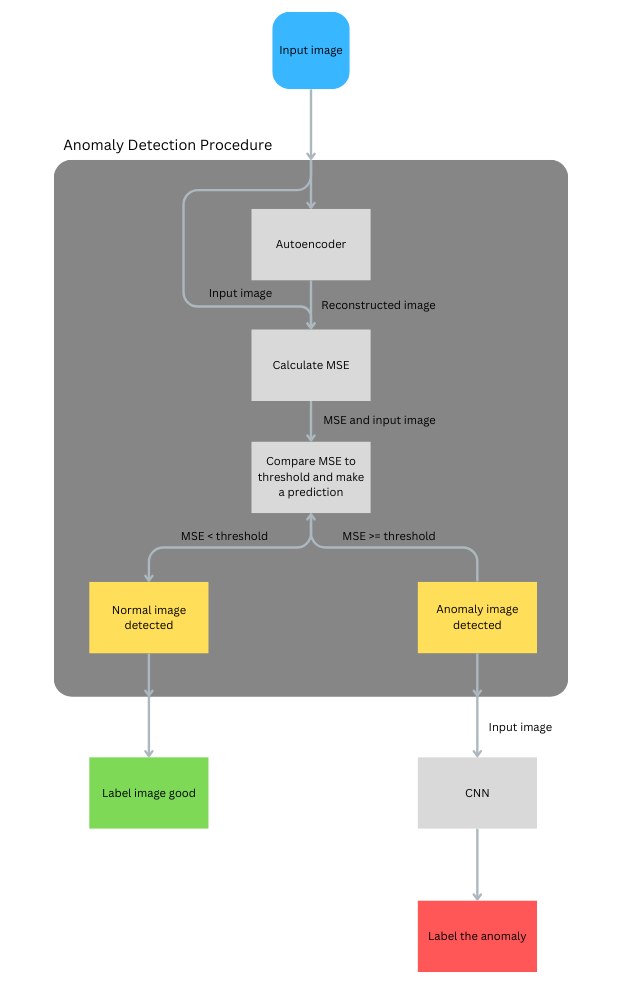
\includegraphics[scale=0.6]{src/images/machine_learning_pipeline.png}
    \caption{Machine learning pipeline visualized}
    \label{fig:ml_pipeline}
\end{figure}
\par
Opt 2:
\par
Our model pipeline consists of two models: a CNN and an Autoencoder. 
The Autoencoder first detects and highlights anomalies in the input images. These processed images are then fed into the CNN, which classifies them into one of our four possible classes.
The pipeline outputs both the processed image with highlighted anomalies and its corresponding classification label, providing great analysis of bottle defects.

\subsection{Autoencoder}

\subsection{Anomaly detection procedure}

\subsection{CNN}

\subsubsection{Introducing noise}
To ensure model robustness in real-world conditions, we introduced two types of noise to the images: Gaussian noise and Salt and Pepper noise. 
Gaussian noise simulates random intensity variations that might occur due to poor lighting or sensor noise, while Salt and Pepper noise represents random white and black pixels that could appear due to dead pixels or transmission errors.
Additionally, we introduced noise by flipping and rotating images, which simulates diffrent camera angels and orientations.

\begin{figure}[H]
    \centering
    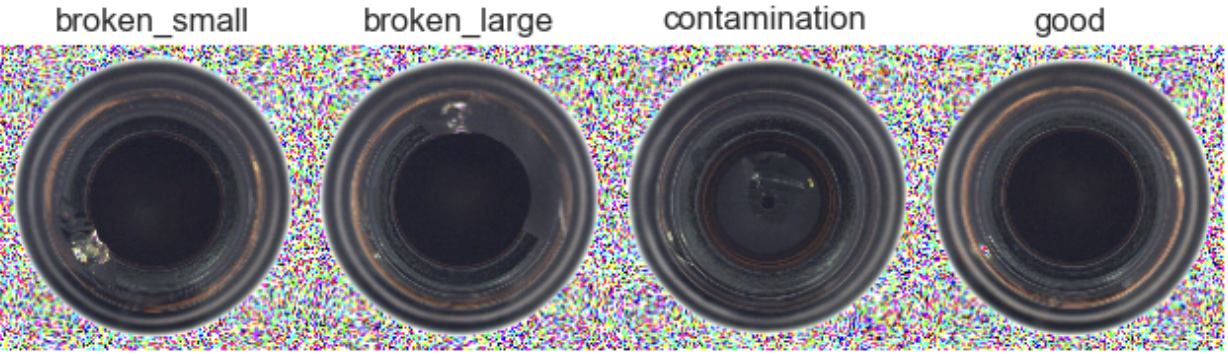
\includegraphics[scale=0.55]{src/images/dataset_w_gnoise.png}
    \caption{Images with Gaussian noise.}
    \label{fig:Gnoise}
\end{figure}
\begin{figure}[H]
    \centering
    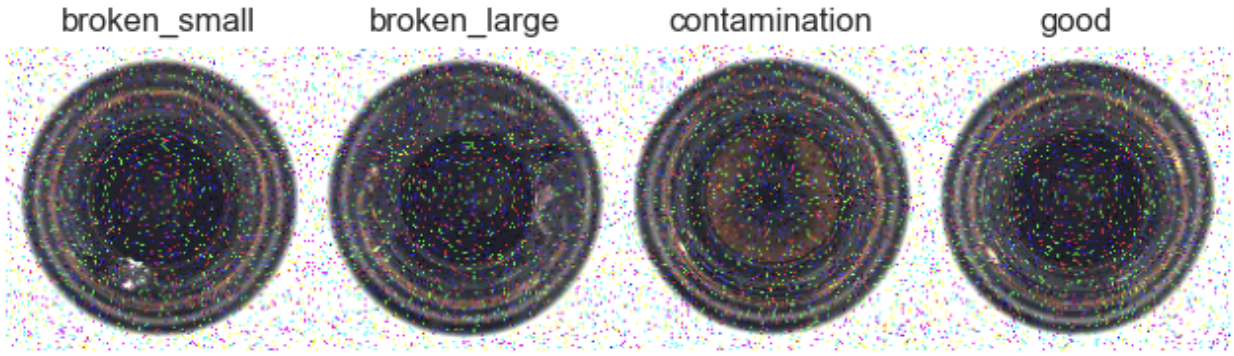
\includegraphics[scale=0.55]{src/images/dataset_w_snp.png}
    \caption{Images with Salt and Pepper noise.}
    \label{fig:snpnoise}
\end{figure}

\subsubsection{Implemention of the CNN} % Ha denna under CNN-section och bara kalla Implementation?
The CNN model is implemented using TensorFlow's Sequential API with the following architecture:
\vspace{0.3cm}
\begin{python}
model = models.Sequential([
    layers.InputLayer(shape=(150, 150, 3)), 
    layers.Conv2D(32, (3, 3), activation='relu', padding='same', strides=(2, 2)),
    layers.MaxPooling2D((2, 2)),
    layers.Conv2D(64, (3, 3), activation='relu', padding='same', strides=(2, 2)),
    layers.MaxPooling2D((2, 2)),
    layers.Conv2D(128, (3, 3), activation='relu', padding='same', strides=(2, 2)),
    layers.MaxPooling2D((2, 2)),
    layers.Flatten(),
    layers.Dense(128, activation='relu'),
    layers.Dense(4, activation='softmax')
])
model.compile(
    optimizer='adam',
    loss='categorical_crossentropy',
    metrics=['accuracy']
)
\end{python}

The model consists of three convolutional layers, each followed by max pooling layers, and two dense layers for classification. The input images are 150x150 pixels with 3 color channels.
\subsubsection{Implemention of the Autoencoder}

